\documentclass{beamer}
\usepackage{lmodern}
\usepackage[utf8]{inputenc}
\usepackage{hyperref}
\usepackage{minted}
\usepackage{color}
\usepackage{booktabs}
\usepackage{tabularx}
\usepackage{array}
\usepackage{graphicx}

\setbeamertemplate{navigation symbols}{}
\mode<presentation>{\usetheme{Madrid}}

\title{Named Entity Classification}   
\author{Madita Huvar, Sanaz Safdel, Phillip R.-P.} 
\date{\today} 

\begin{document}



\begin{frame}
\titlepage
\end{frame} 

\begin{frame}
\frametitle{Inhaltsverzeichnis}
\tableofcontents
\end{frame} 


\section{Einführung}
\begin{frame}
	\frametitle{NER in der Forschung}
	Named Entity Recognition seit 1990er Jahren aktives Forschungsfeld. (Überblick: Borthwick, 1999, Tjong Kim Sang 2003, Marrero 2012)\\
	
	Grundlage für weitere Forschungsfelder im Bereich Information Retrieval, z.B. Semantic Annotation, Question Answering, Opinion Mining, usw. (Marrero 2012)
\end{frame}
\begin{frame}
	\frametitle{Was sind Named Entities}
	Named Entities sind Phrasen die Namen von Personen, Organisationen, Währungen, usw enthalten. Beispiele:\\
	
	[ORG U.N. ], [PER Obama ], [MONEY Dollar], [LOC Moscow ] 
\end{frame}
	\begin{frame}
		\frametitle{Unser Projekt}
		\begin{itemize}
			\item Typischerweise werden Named Entity Recognition und Named Entity Classification (NEC) zusammen betrachtet.
			\item Wenige Untersuchungen beschäftigen sich nur mit NEC. (Primadhanty 2014, He 2016, Spangler 2016)
			\item Dieses Projekt konzentriert sich auf NEC und stellt die Frage, welchen Einfluss Feature Selection auf die Klassifikationsergebnisse eines Nemed Entity Klassifizierers hat.
			\item 		Untersuchung konzentriert sich auf einfache syntaktische und lexikalische Features, die in fast allen Forschungsarbeiten in ähnlicher Form genutzt wurden. \textit{(Toral, Munoz, 2006; Kazama, Torisawa, 2007; Ratinov, Roth 2009)} 
		\end{itemize}	

	\end{frame}
\section{Daten \& Tools}
	\subsection{Tools}
	\begin{frame}
			\frametitle{Tools}
			\begin{itemize}
				\item Python 3.4+
				\item Scikit Learn als Klassifizierer
				\item liac-arff
				\item matplotlib
				\item Weka zur Korpusanalyse
			\end{itemize}
	\end{frame}
	\subsection{Korpus}
	\begin{frame}
			\frametitle{Korpus}
			\begin{itemize}
				\item Für Named Entity Klassifikation wird OntoNotes Korpus 2012 genutzt. \textit{(OntoNotes Release 5.0 2012)}
				\item Englischen Nachrichtentexte des 'The Wall Street Journal'.
				Für die Entwicklungsphase bereits vorgefertigtes Developmenttest.
				\item Für die Klassifikation der Named Entities werden die bereits vorgefertigten Trainings- und Testdatensets genutzt.
			\end{itemize}
			 \begin{table}
			 	\caption{Anzahl an atomaren Named Entities}
			 	\begin{tabular}{ccc}
			 		\toprule
					Developmentset & Trainingset & Testset\\
			 		\midrule
					3325 & 23686 & 2996\\
			 		\bottomrule
			 	\end{tabular}
			 	\label{tab:datasets}
			 \end{table}
	\end{frame}
		\begin{frame}
			\frametitle{Korpusreader}
			\begin{itemize}
				\item Für Extraktion der Named Entities wurde ein Korpusreader erstellt.
				\item 	Der Reader extrahiert alle Named Entities, inklusive POS-tags der einzelnen Token, Phrasenart, Kontextwörtern (ne-1, ne+1), und ordnet sie Klassen zu.
			\end{itemize}
			
			
		
			
			Beispiel:\\
			\{'PERSON':[['Peter', 'NNP'],['Mokaba', 'NNP'],'NP', ('Says', ',')]\}
		\end{frame}
	
	\subsection{Korpusklassen}
		\begin{frame}
			\frametitle{Korpusklassenbalancierung}
				\begin{table}
				\caption{Klassen im OntoNotes Korpus \textit{(OntoNotes Release 5.0 2012)}}
				\begin{tabularx}{\textwidth}{Xc}
					\toprule
					Klassen  & Trainingset \\
					\midrule
					ORG  & 5788 \\
					PERSON & 3756 \\
					GPE & 3601 \\
					NORP & 1484 \\
					PERCENT & 1061  \\
					CARDINAL & 1852 \\
					MONEY & 1509  \\
					DATE & 4080  \\
					FAC, LOC, PRODUCT, EVENT, WORK\_OF\_ART, LAW, LANGUAGE, TIME, QUANTITY, ORDINAL & $<$ 1800 \\
					\bottomrule
				\end{tabularx}
				\label{tab:datasets}
			\end{table}
		\end{frame}
	\begin{frame}
		\frametitle{Beschreibung Korpusklassen}
		\begin{table}
			\caption{Balancierte Klassen}
			\begin{tabularx}{\textwidth}{lX}
				\toprule
				Klassen  & Beschreibung \\
				\midrule
				PERSON 	& People, including fictional \\
				NORP\_GPE &	Nationalities or religious or political groups
				Countries, cities, states\\
				ORGANIZATION &	Companies, agencies, institutions, etc.\\
				DATE &	Absolute or relative dates or periods\\
				PERCENT\_MONEY\_CARDINAL &	Percentage (including “\%”)
				Monetary values, including unit
				Numerals that do not fall under another type \\
				\bottomrule
			\end{tabularx}
			\label{tab:datasets}
		\end{table}
	\end{frame}
	
	\begin{frame}
			\frametitle{Verteilung Korpusklassen}
			 \begin{table}
			 	\caption{Verteilung der Klassen nach Balancierung}
			 	\begin{tabular}{lccc}
			 		\toprule
			 		Klassen  & Developmentset & Trainingset & Testset \\
			 		\midrule
			 		ORG  & 930 & 5857 & 859 \\
			 		PERSON & 486 & 3759 & 413 \\
			 		GPE\_NORP & 732 & 5134 & 588 \\
			 		PERCENT\_CARDINAL\_MONEY & 564 & 4672 & 529 \\
			 		DATE & 613 & 4254 & 601 \\
			 		\bottomrule
			 	\end{tabular}
			 	\label{tab:datasets}
			 \end{table}
	\end{frame}


\section{Klassifizierer}
	\subsection{Features für den Baseline-Klassifizierer}
	\begin{frame}
		\frametitle{Features für den Baseline-Klassifizierer}
		Anzahl der Features: 1317
					 \begin{table}
					 	\caption{Features für den Baseline-Klassifizierer}
					 	\begin{tabularx}{\textwidth}{llX}
					 		\toprule
							Feature & Wert & Beschreibung\\
					 		\midrule
					 		Unigram & numerisch & Vorkommen der Unigramme, die mindestens fünfmal im Trainingscorpus vorkommen. \textit{(Mayfield 2003)} \\
					 		\bottomrule
					 	\end{tabularx}
					 	\label{tab:baselinef}
					 \end{table}
	\end{frame}
	\subsection{Erweitertes Featureset}
	\begin{frame}
		\frametitle{Erweitertes Featureset I}
		Anzahl der Features: 1716
 			\begin{table}
 				\caption{Features für den Klassifizierer I}
 				\begin{tabularx}{\textwidth}{llX}
 					\toprule
 					Feature & Wert & Beschreibung\\
 					\midrule
 					Unigram & numerisch & Vorkommen der Unigramme (lemmatisiert), die mindestens fünfmal im Trainingscorpus vorkommen. \textit{(Mayfield 2003)}\\
 					POS & numerisch & Häufigkeit von 36 POS-Tags aus der Penn Treebank \textit{(Florian, Chieu 2003)}\\
 					isAllCaps & boolean & Wörter nur in Großschreibung \textit{(Nadeau 2006)}\\
 					Context & numerisch & Vorkommen der Kontexttokens, die mindestens fünfmal im Trainingskorpus vorkommen. Das Kontextfenster beinhaltet das Vorgänger- und Nachfolgetoken der NE. \textit{(Munro 2003)}\\
 					containsDigit & boolean & Vorkommen von Nummern. \textit{}\\
 					\bottomrule
 				\end{tabularx}
 				\label{tab:allf1}
 			\end{table}
 	\end{frame}
 		\begin{frame}
 			\frametitle{Erweitertes Featureset II}
 					\begin{table}
 						\caption{Features für den  Klassifizierer II}
 						\begin{tabularx}{\textwidth}{llX}
 							\toprule
 							Feature & Wert & Beschreibung\\
 							\midrule
 							isInWiki & boolean & Vorkommen der NE in der Wikipedia. \textit{(Toral and Munoz, 2006; Kazama and Torisawa, 2007)}\\
 							isTitle & boolean & Prüft, ob Titelbezeichnungen (z.B. Mr. MA) vorkommen. \textit{Ratinov, Roth 2009}\\
 							isNP & boolean & Ist NE eine Nominalphrase. \textit{Sánchez, Cuadrado 2009}\\
 							isName & boolean & Prüft, ob Vornamen vorkommen.\textit{Ratinov, Roth 2009}\\
 							containsDash & boolean & Vorkommen von Viertelgeviertstrichen. \textit{Mayfield 2003}\\
 							\bottomrule
 						\end{tabularx}
 						\label{tab:allf2}
 					\end{table}
 		\end{frame}
	\subsection{Klassifizierertyp}
	\begin{frame}
		\frametitle{Klassifizierertyp}
		Zur Klassifizierung der NE wird eine Support Vector Maschine mit linearem Kernel verwendet.\\
		
		\textit{Alternativ wurde ein Decisiontree getestet, dieser hatte allerdings mit allen Featurekombinationen tendenziell schlechtere Evaluationsergebnisse. Zudem trainiert der SVM deutlich schneller.}\\
		
		\begin{itemize}
			\item SVM (sklearn.svm.LinearSVC)\\
			
				Featurevektoren haben sehr viele Features
				daher linearer Kernel.\\
				Mapping in höheren Featurespace eines nicht-linearen Kernels bringt kaum Klassifizierungsverbesserungen. \textit{(Chih-Wei Hsu 2003)}\\
		\end{itemize}
	\end{frame}

	\subsection{Erfahrungen mit den Korpusklassen}
	\begin{frame}
		\frametitle{Erfahrungen mit den Korpusklassen I}
		Wie die ROC-Kurve zeigt, hat der Klassifizierer insbesondere Schwierigkeiten, die Klassen PERSON und ORG und GPE\_NORP zu unterscheiden.\\
	\end{frame}
	\begin{frame}
		\frametitle{ROC Curve}
		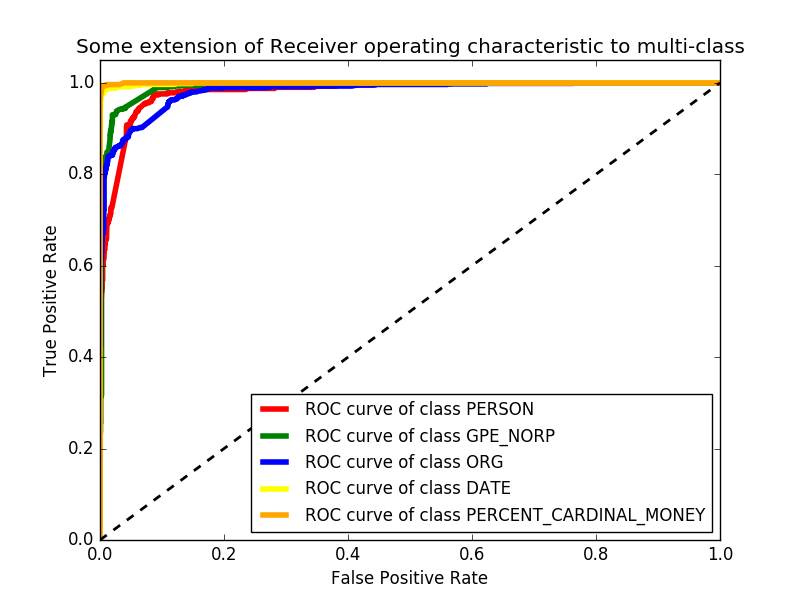
\includegraphics[scale=0.3]{roc_curve.png}
	\end{frame}
		\begin{frame}
			\frametitle{Erfahrungen mit den Korpusklassen II}
			Die Confusion Matrix zeigt, dass von den 361 PERSON Entities, 71 als ORG und 29 als GPE\_NORP klassifiziert werden. 
			\begin{table}
				\caption{Confusion Matrix}
				\begin{tabularx}{\textwidth}{llllll}
					\toprule
					361 & 28 & 22 & 2 & 0 & PERSON\\
					29 & 549 & 10 & 0 & 0 & GPE\_NORP\\
					71 & 45 & 736 & 6 & 1 & ORG\\
					0 & 2 & 1 & 591 & 7 & DATE\\
					0 & 2 & 0 & 2 & 525 & PERCENT\_CARDINAL\_MONEY\\
					\bottomrule
				\end{tabularx}
				\label{tab:allf2}
			\end{table}			
		\end{frame}

\section{Evaluation}
	\begin{frame}
		\frametitle{Featureselektion I}
		Insgesamt haben werden elf Features eingesetzt.\\
		
		Um die Performance der einzelnen Features zu testen, wurde die Potenzmenge des Featuresets gebildet.\\
		
		Schließlich wurde der Klassifizierer auf allen 1013 Teilmengen durchgeführt.\\
	\end{frame}
	\begin{frame}
		\frametitle{Featureselektion II}
			Für die Evaluation entscheidend waren alle Teilmengen, die die Features 'Unigram' und 'Context' enthalten und mind. drei Features 3 besitzen.\\
					
			\begin{itemize}
				\item Accuracy aller Teilnmengen ohne diese Features: \textless 69 \%.
				\item Accuracy nur mit Unigram und Context: 87.42\%
			\end{itemize}

					
	\end{frame}
		\begin{frame}
			\frametitle{Featureselektion III}
			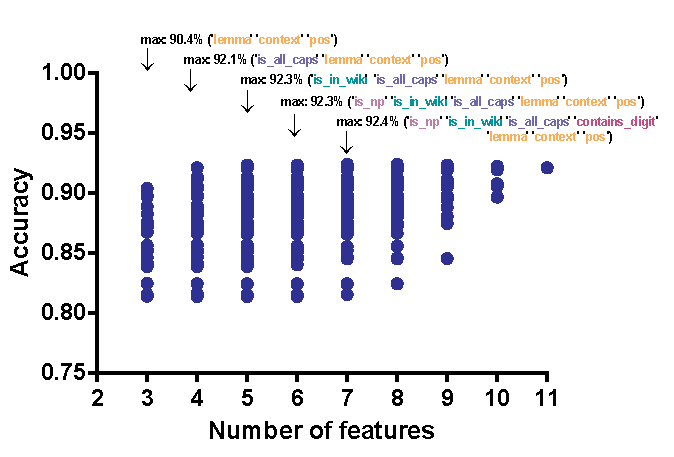
\includegraphics[scale=0.9]{accuracy.pdf}\\

		\end{frame}
	\begin{frame}
		\begin{itemize}
			\item Beste Features: 'Unigram', 'Context'\\
			\item Höchste Accuracy: Ab sieben Features.\\
			\item Weitere Features:\\
		\end{itemize}
	\end{frame}
	\begin{frame}
		\frametitle{Evaluation}
		Hier kommt ein eval\_report hin mit Accuracy-Wert und eine Grafik/Tabelle, die die wichtigsten Features anzeigt.\\
		Tabelle mit Baseline Eval lemma + context Eval und Fullfeature Eval.\\
				\begin{table}
					\caption{Final Evaluation}
					\begin{tabularx}{\textwidth}{llll}
						Featureset & & Accuracy & F1-Score\\
						\toprule
						Baseline & unbalanced & 0.786757848928 &  0.786781978815\\
								 & balanced & 0.840802675585 & 0.854079560307\\
						Best	 & unbalanced & 0.87286291576 & 0.869301986664\\
								 & balanced & 0.923745819398 & 0.924314367424\\
						\bottomrule
					\end{tabularx}
					\label{tab:allf2}
				\end{table}	
		
		
		
		
	\end{frame}
		\subsection{Probleme}
		\begin{frame}
			\frametitle{Probleme}
			Context bezieht auch Satzzeichen ein (oft ',' oder '.'), dies könnte man auf alphanumerische Strings beschränken.\\
			
			Klassifikationsfehler im Testset, da nur die automatisch annotierte Testsetversion von OntoNotes v5 zur Verfügung steht.\\
			
			Beispiel:\\
			\{'ORG': [['American', 'JJ'], 'NP', ('to', 'notions')]\}\\classified as ['GPE\_NORP']\\
			
		\end{frame}
\section{Ausblick}
	\begin{frame}
		\frametitle{Ausblick}
		Was kann man noch verbessern?
	\end{frame}
\section{Referenzen}
	\begin{frame}
		\frametitle{Referenzen}
		\begin{itemize}
			\item Cho, Han-Cheol; Okazaki, Naoaki; Miwa, Makoto; Tsujii, Jun’ichi (2013): Named entity recognition with multiple segment representations. In: Information Processing \& Management 49\\
			\item Derczynski, Leon; Maynard, Diana; Rizzo, Giuseppe; van Erp, Marieke; Gorrell, Genevieve; Troncy, Raphaël et al. (2015): Analysis of named entity recognition and linking for tweets. In: Information Processing \& Management 51 (2), S. 32–49.\\
			\item Konkol, Michal; Brychcín, Tomáš; Konopík, Miloslav (2015): Latent semantics in Named Entity Recognition. In: Expert Systems with Applications 42 (7), S. 3470–3479.\\
			\item Agerri, Rodrigo; Rigau, German (2016): Robust multilingual Named Entity Recognition with shallow semi-supervised features. In: Artificial Intelligence 238, S. 63–82.\\
			\item Erik F. Tjong Kim Sang and Fien De Meulder (2003): Language-Independent Named Entity Recognition.\\
		\end{itemize}
	\end{frame}
	\begin{frame}
		\begin{itemize}
			\item Marrero, Mónica; Urbano, Julián; Sánchez-Cuadrado, Sonia; Morato, Jorge; Gómez-Berbís, Juan Miguel (2013): Named Entity Recognition. Fallacies, challenges and opportunities. In: Computer Standards \& Interfaces 35 (5), S. 482–489.\\
			\item Mayfield, James; McNamee, Paul; Piatko, Christine (2003): Named entity recognition using hundreds of thousands of features. In: Walter Daelemans und Miles Osborne (Hg.): Proceedings of the seventh conference on Natural language learning at HLT-NAACL 2003 -. the seventh conference. Edmonton, Canada. Morristown, NJ, USA: Association for Computational Linguistics, S. 184–187.\\
			\item Mónica Marrero, Sonia Sánchez-Cuadrado (2009): Evaluation of Named Entity Extraction Systems.\\
			\item Weischedel, Ralph M. (2013): OntoNotes release 5.0. [Philadelphia, Pa.]: Linguistic Data Consortium.\\
		\end{itemize}
	\end{frame}

\end{document}
